\documentclass{beamer}
\mode<presentation>
\usepackage{amsmath}
\usepackage{amssymb}
%\usepackage{advdate}
\usepackage{adjustbox}
\usepackage{subcaption}
\usepackage{enumitem}
\usepackage{multicol}
\usepackage{listings}
\usepackage{url}
\def\UrlBreaks{\do\/\do-}
\usepackage{ifpdf}

\usetheme{AnnArbor}
\usecolortheme{lily}
\setbeamertemplate{footline}
{
  \leavevmode%
  \hbox{%
  \begin{beamercolorbox}[wd=\paperwidth,ht=2.25ex,dp=1ex,right]{author in head/foot}%
    \insertframenumber{} / \inserttotalframenumber\hspace*{2ex} 
  \end{beamercolorbox}}%
  \vskip0pt%
}
\setbeamertemplate{navigation symbols}{}

\providecommand{\nCr}[2]{\,^{#1}C_{#2}} % nCr
\providecommand{\nPr}[2]{\,^{#1}P_{#2}} % nPr
\providecommand{\mbf}{\mathbf}
\providecommand{\pr}[1]{\ensuremath{\Pr\left(#1\right)}}
\providecommand{\qfunc}[1]{\ensuremath{Q\left(#1\right)}}
\providecommand{\sbrak}[1]{\ensuremath{{}\left[#1\right]}}
\providecommand{\lsbrak}[1]{\ensuremath{{}\left[#1\right.}}
\providecommand{\rsbrak}[1]{\ensuremath{{}\left.#1\right]}}
\providecommand{\brak}[1]{\ensuremath{\left(#1\right)}}
\providecommand{\lbrak}[1]{\ensuremath{\left(#1\right.}}
\providecommand{\rbrak}[1]{\ensuremath{\left.#1\right)}}
\providecommand{\cbrak}[1]{\ensuremath{\left\{#1\right\}}}
\providecommand{\lcbrak}[1]{\ensuremath{\left\{#1\right.}}
\providecommand{\rcbrak}[1]{\ensuremath{\left.#1\right\}}}
\theoremstyle{remark}
\newtheorem{rem}{Remark}
\newcommand{\sgn}{\mathop{\mathrm{sgn}}}
\providecommand{\res}[1]{\Res\displaylimits_{#1}} 
\providecommand{\norm}[1]{\lVert#1\rVert}
\providecommand{\mtx}[1]{\mathbf{#1}}
\providecommand{\fourier}{\overset{\mathcal{F}}{ \rightleftharpoons}}
%\providecommand{\hilbert}{\overset{\mathcal{H}}{ \rightleftharpoons}}
\providecommand{\system}{\overset{\mathcal{H}}{ \longleftrightarrow}}
%\newcommand{\solution}[2]{\textbf{Solution:}{#1}}
%\newcommand{\solution}{\noindent \textbf{Solution: }}
\providecommand{\dec}[2]{\ensuremath{\overset{#1}{\underset{#2}{\gtrless}}}}
\newcommand{\myvec}[1]{\ensuremath{\begin{pmatrix}#1\end{pmatrix}}}
\let\vec\mathbf

\lstset{
%language=C,
frame=single, 
breaklines=true,
columns=fullflexible
}



\title{Presentation on problem 15}
\author{Kalepalli.N V S D M Ananyan\\EE19BTECH11013\\ Dept. of Electrical Engg.,\\IIT Hyderabad }

\date{\today}










\usepackage{graphicx}               % Necessary to use \scalebox
\usepackage{amsmath,amssymb}

\begin{document}

\begin{frame}
\titlepage
\end{frame}









\section*{Outline}
\begin{frame}
\tableofcontents
\end{frame}










\section{Problem}
\subsection{Problem Statement}
\begin{frame}
\frametitle{Problem Statement}

 Use MATLAB and the Symbolic Math Symbolic Math Toolbox to input and form LTI objects in polynomial and factored form for the following frequency functions:

\begin{equation}
\vec{a)}. \vec{G(s)} = \frac{45(s^2+37s+74)(s^3+28s^2+32s+16)}{(s+39)(s+47)(s^2+2s+100)(s^3+27s^2+18s+15)}
\end{equation}

\begin{equation}
\vec{b)}. \vec{G(s)} = \frac{56(s+14)(s^3+49s^2+62s+53)}{(s^3+81s^2+76s+65)(s^2+88s+33)(s^2+56s+77)}
\end{equation}

\end{frame}












\section{Solution for part (a)}

\subsection{Polynomial form of G(s)}
\begin{frame}
\frametitle{Polynomial form of G(s)}
\begin{enumerate}[label=(\roman*)]
\begin{description}
    \item[$\bullet$]From the expanded form of numerator and denominator, we can write polynomial form of transfer function as:
\end{description}

\vspace{0.2 in}
\noindent 
 $ {\textsyle \frac{45s^5+2925s^4+53190s^3+147240s^2+133200s+53280}{s^7+115s^6+4499s^5+70700s^4+553692s^3+5201463s^2+3483390s+2749500}} $\\
\noindent
\vspace{0.1 in}

\end{enumerate}
\end{frame}











\subsection{Poles and zeroes}
\begin{frame}
\frametitle{Poles and zeroes of G(s)}
\begin{description}
\item[$\bullet$]We can obtain the roots of a polynomial using numpy library in python3.
\item[$\bullet$]Using numpy, we find roots of numerator which are the zeroes and roots of denominator which are the poles of Transfer function.
\item[$\bullet$]Poles of the transfer function are:\\
1)-47\\
2)-39\\
3)-26.34\\
4)-1+9.95j\\
5)-1-9.95j\\
6)-0.33+0.68j\\
7)-0.33-0.68j\\
\vspace{0.1 in}
where j is the square root of -1
\end{description}
\end{frame}

\begin{frame}
\frametitle{Poles and zeroes of G(s)}
\begin{description}
\item[$\bullet$]Similarly, we can obtain roots of numerator also.
\item[$\bullet$]Zeroes of the transfer function are:\\
1)-34.88\\
2)-26.83\\
3)-2.12\\
4)-0.59+0.5j\\
5)-0.59-0.5j\\

\vspace{0.1 in}
where j is the square root of -1
\end{description}
\end{frame}












\subsection{Factored form of G(s)}
\begin{frame}
\frametitle{Factored form of G(s)}
\begin{description}
\item[$\bullet$]From the obtained values of poles and zeroes, we can write factored form of the Transfer function as :
\end{description}
\vspace{0.2 in}
\noindent 
 $ {\textsyle \frac{(s+34.88)(s+26.83)(s+2.12)(s+0.59-0.5j)(s+0.59+0.5j)}{(s+47)(s+39)(s+26.34)(s+1-9.95j)(s+1+9.95j)(s+0.33-0.68j)(s+0.33+0.68j)}} $\\
\noindent
\vspace{0.1 in}

\end{frame}























\section{Solution for part (b)}

\subsection{Polynomial form of G(s)}
\begin{frame}
\frametitle{Polynomial form of G(s)}
\begin{enumerate}[label=(\roman*)]
\begin{description}
    \item[$\bullet$]From the expanded form of numerator and denominator, we can write polynomial form of transfer function as:
\end{description}

\vspace{0.2 in}
\noindent 
 $ {\textsyle \frac{56s^4+3528s^3+41888s^2+51576s+41552}{s^7+225s^6+16778s^5+427711s^4+1093333s^3+1188715s^2+753676s+165165}} $\\
\noindent
\vspace{0.1 in}

\end{enumerate}
\end{frame}











\subsection{Poles and zeroes}
\begin{frame}
\frametitle{Poles and zeroes of G(s)}
\begin{description}
\item[$\bullet$]We can obtain the roots of a polynomial using numpy library in python3.
\item[$\bullet$]Using numpy, we find roots of numerator which are the zeroes and roots of denominator which are the poles of Transfer function.
\item[$\bullet$]Poles of the transfer function are:\\
1)-87.62\\
2)-80.06\\
3)-54.59\\
4)-1.41\\
5)-0.47+0.77j\\
6)-0.47-0.77j\\
7)-0.38\\
\vspace{0.1 in}
where j is the square root of -1
\end{description}
\end{frame}


\begin{frame}
\frametitle{Poles and zeroes of G(s)}
\begin{description}
\item[$\bullet$]Similarly, we can obtain roots of numerator also.
\item[$\bullet$]Zeroes of the transfer function are:\\
1)-47.72\\
2)-14\\
3)-0.64+0.84j\\
4)-0.64-0.84j\\

\vspace{0.1 in}
where j is the square root of -1
\end{description}
\end{frame}









\subsection{Factored form of G(s)}
\begin{frame}
\frametitle{Factored form of G(s)}
\begin{description}
\item[$\bullet$]From the obtained values of poles and zeroes, we can write factored form of the Transfer function as :
\end{description}
\vspace{0.2 in}
\noindent 
 $ {\textsyle \frac{(s+47.72)(s+14)(s+0.64-0.84j)(s+0.64+0.84j)}{(s+87.62)(s+80.06)(s+54.59)(s+1.41)(s+0.47-0.77j)(s+0.47+0.77j)(s+0.38)}} $\\
\noindent
\vspace{0.1 in}

\end{frame}

















\section{Python codes and Terminal output}

\subsection{Python code for part (a)}
\begin{frame}
\frametitle{Python code for part (a)}
\usepackage{}
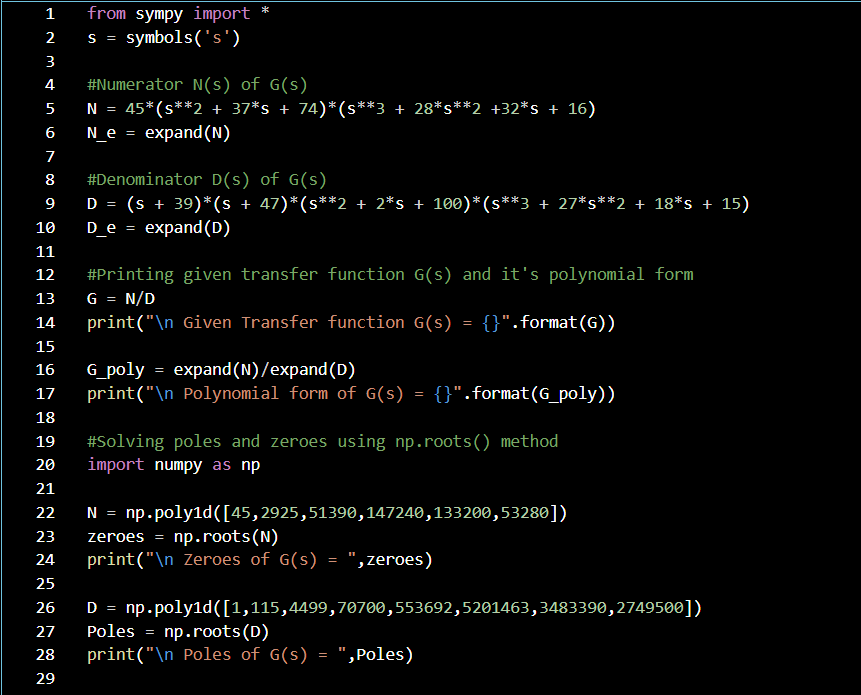
\includegraphics[width=10cm,height=7.5cm]{Assignment 1/15_a.png}
\end{frame}









\subsection{Python code for part (b)}
\begin{frame}
\frametitle{Python code for part (b)}
\usepackage{}
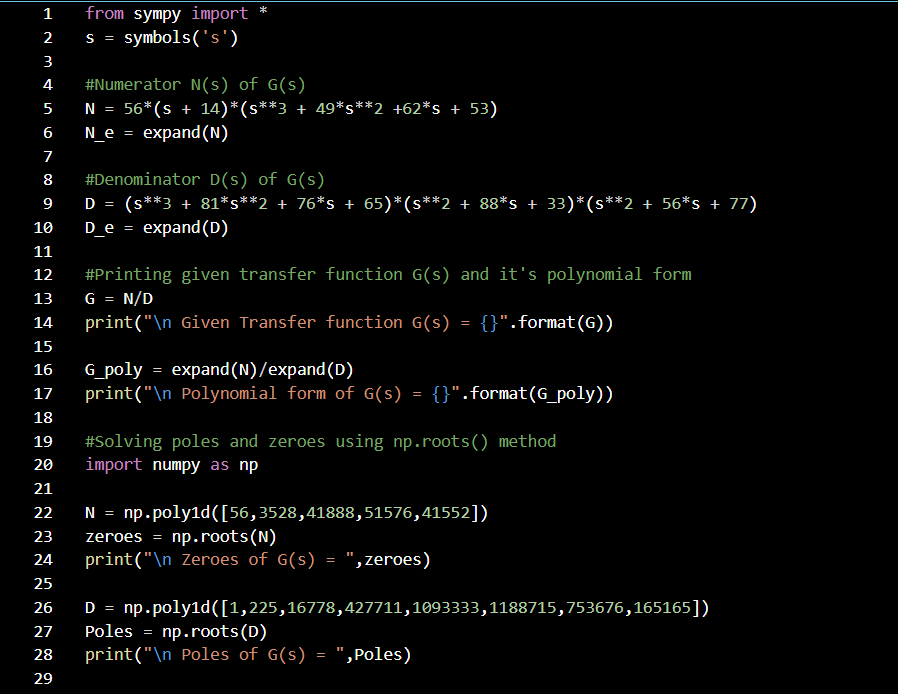
\includegraphics[width=10cm,height=7.5cm]{Assignment 1/15_b.png}

\end{frame}










\subsection{Terminal output}
\begin{frame}
\frametitle{Terminal output }
\usepackage{}
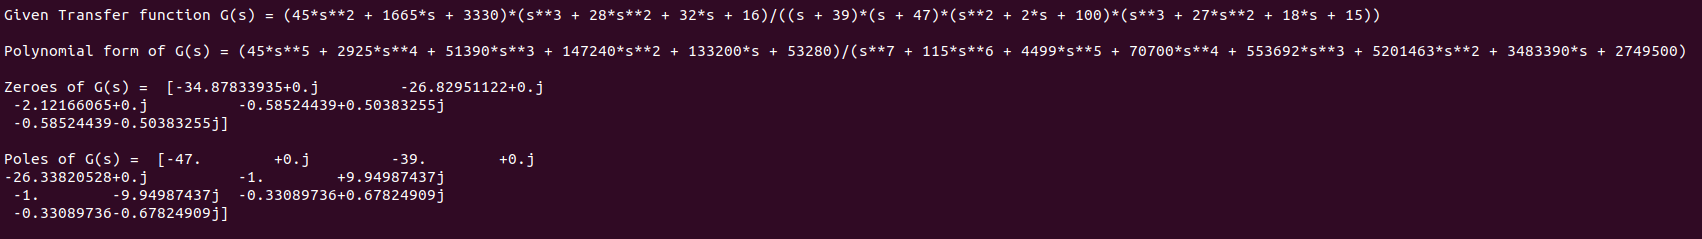
\includegraphics[width=12cm,height=1.9cm]{Assignment 1/15a.png}
\end{frame}











\subsection{Terminal output}
\begin{frame}
\frametitle{Terminal output }
\usepackage{}
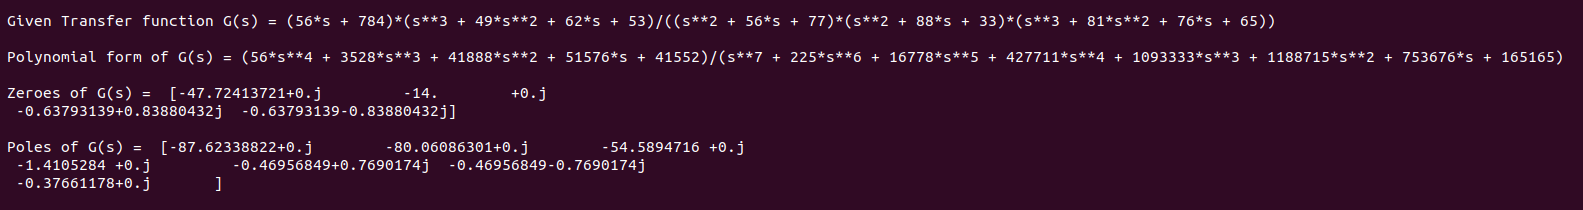
\includegraphics[width=12cm,height=1.9cm]{Assignment 1/15b.png}
\end{frame}










\subsection{Github link}
\begin{frame}
\frametitle{Github link}

The python codes, terminal output pictures, tex document and the pdf file are in the Assignment 1 folder of control systems repository in the below hyper link :\\
\vspace{0.2 in}

\href{https://github.com/KalepalliNVSDMAnanyan/control-systems}{Please click Here}







\end{frame}















%\begin{frame}
%\frametitle{Introduction}
%\framesubtitle{Literature}
%%\begin{figure}[t!]
%%    \centering
%%    \begin{subfigure}[t]{0.4\columnwidth}
%%        \centering
%%        \includegraphics[width=\columnwidth]{point_source}
%%        \caption{Single point source}
%%\label{fig3:subfig1}        
%%    \end{subfigure}%
%%    ~ 
%%    \begin{subfigure}[t]{0.4\columnwidth}
%%        \centering
%%        \includegraphics[width=\columnwidth]{pointNoPowerDist_new}
%%        \caption{SNR profile}
%%\label{fig3:subfig2}
%%    \end{subfigure}
%%  %  \caption{Average SNR for a BPP. $N=16$}
%%    \label{fig3}
%%  \end{figure}
%
%\end{frame}
%  
%
%
%%

\end{document}
